\documentclass[12pt]{article}
\usepackage[margin=1in]{geometry} 
\usepackage{amsmath}
\usepackage{tcolorbox}
\usepackage{amssymb}
\usepackage{amsthm}
\usepackage{lastpage}
\usepackage{fancyhdr}
\usepackage{accents}
\usepackage{mathtools}
\usepackage{tikz}
\usepackage{gensymb}
\usepackage{listings}
\usepackage{graphicx}
\usepackage{circuitikz}
\usepackage{pgfplots}
\pagestyle{fancy}
\setlength{\headheight}{40pt}

\lstset{
  basicstyle=\ttfamily,
  columns=fullflexible,
  frame=single,
  breaklines=true,
  postbreak=\mbox{\textcolor{red}{$\hookrightarrow$}\space},
}

\newenvironment{solution}
  {\renewcommand\qedsymbol{$\blacksquare$}
  \begin{proof}[Solution]}
  {\end{proof}}
\renewcommand\qedsymbol{$\blacksquare$}

\newcommand{\ubar}[1]{\underaccent{\bar}{#1}}

\usetikzlibrary{calc,patterns,angles,quotes}
\usepackage{amsmath}

\title{Quantitative Engineering Analysis \\ Gauntlet Challenge: Mapping and Path Planning (Level 3)}

\author{Rohil Agarwal, Wesley Soo-Hoo \\ Olin College of Engineering \\ ENGX2001 Spring 2020}
\date{\today}

\begin{document}
\begin{titlepage}
\maketitle

\begin{center}
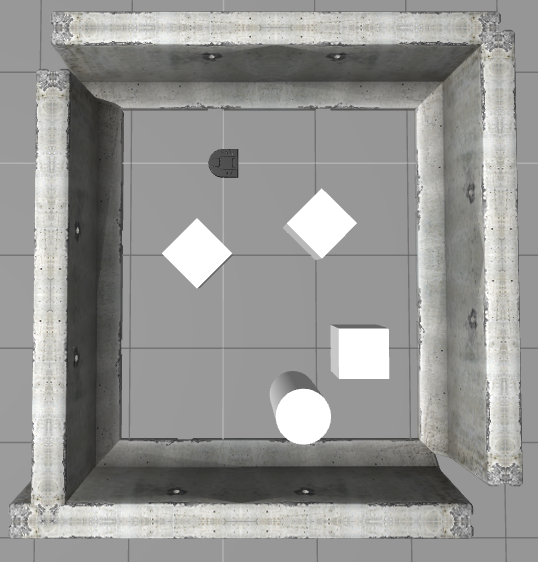
\includegraphics[width=.75\textwidth]{img/CaptureGauntletCover.PNG}
\end{center}
\end{titlepage}



\section{Map}

\begin{figure}[h]
    \centering
    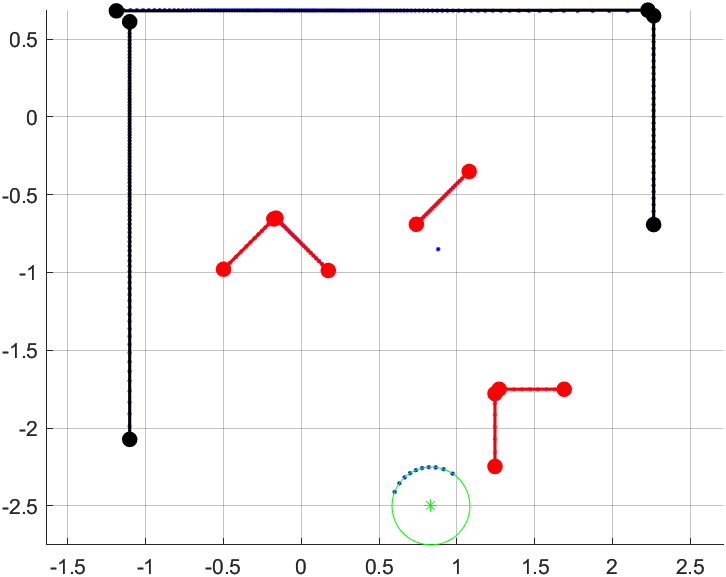
\includegraphics[width=0.65\textwidth]{img/all_shapes.png}
    \caption{Map of the pen, based on a single LIDAR scan obtained from the robot's initial position, with walls and obstacles fitted as line segments and the BoB fitted as a circle.}
    \label{fig:map}
\end{figure}



\section{Potential and Vector Fields}

The Neato traversed a predetermined path that was generated based on the gradient of the potential field given by an equation that mathematically describes the Gauntlet features as sources and sinks. The equation of the potential field, which was based on the intial LIDAR scan, was given by the function

\begin{align*}
    \boldsymbol{f}(x,y) = -&\boldsymbol{w_1}(\ln{\sqrt{(x-x_c)^2+(y-y_c)^2}})\,+ \\
    &\boldsymbol{w_2}(\ln{\sqrt{(x-x_{wp})^2+(y-y_{wp})^2}})\,+ \\
    &\boldsymbol{w_3}(\ln{\sqrt{(x-x_{op})^2+(y-y_{op})^2}})
\end{align*}

\vspace{.1in}

Where:

\begin{itemize}
    \item $w_1$, $w_2$, $w_3$ are the weights for the BoB, wall points, and obstacle points
    \item $x_c$, $y_c$ are the coordinates of the center of the BoB's 
    \item $x_{wp}$, $y_{wp}$ are the coordinates of the points that make up the walls
    \item $x_{op}$, $y_{op}$ are the coordinates of the points that make up the obstacles 
\end{itemize}

In reality, the equation we used included additional versions of the second and third addends for each of the points in the wall and obstacles, respectively. This was because, unlike the BoB the walls and obstacles did not have center points that could be used to sum up the potential field created by the feature. The weights allowed us to adjust the impact of these addends accordingly (BoB addend was given a much larger weight than the addends for each of the points that made up the walls and obstacles). We used for loops to add these additional addends to the function.

\begin{figure}[h!]
    \centering
    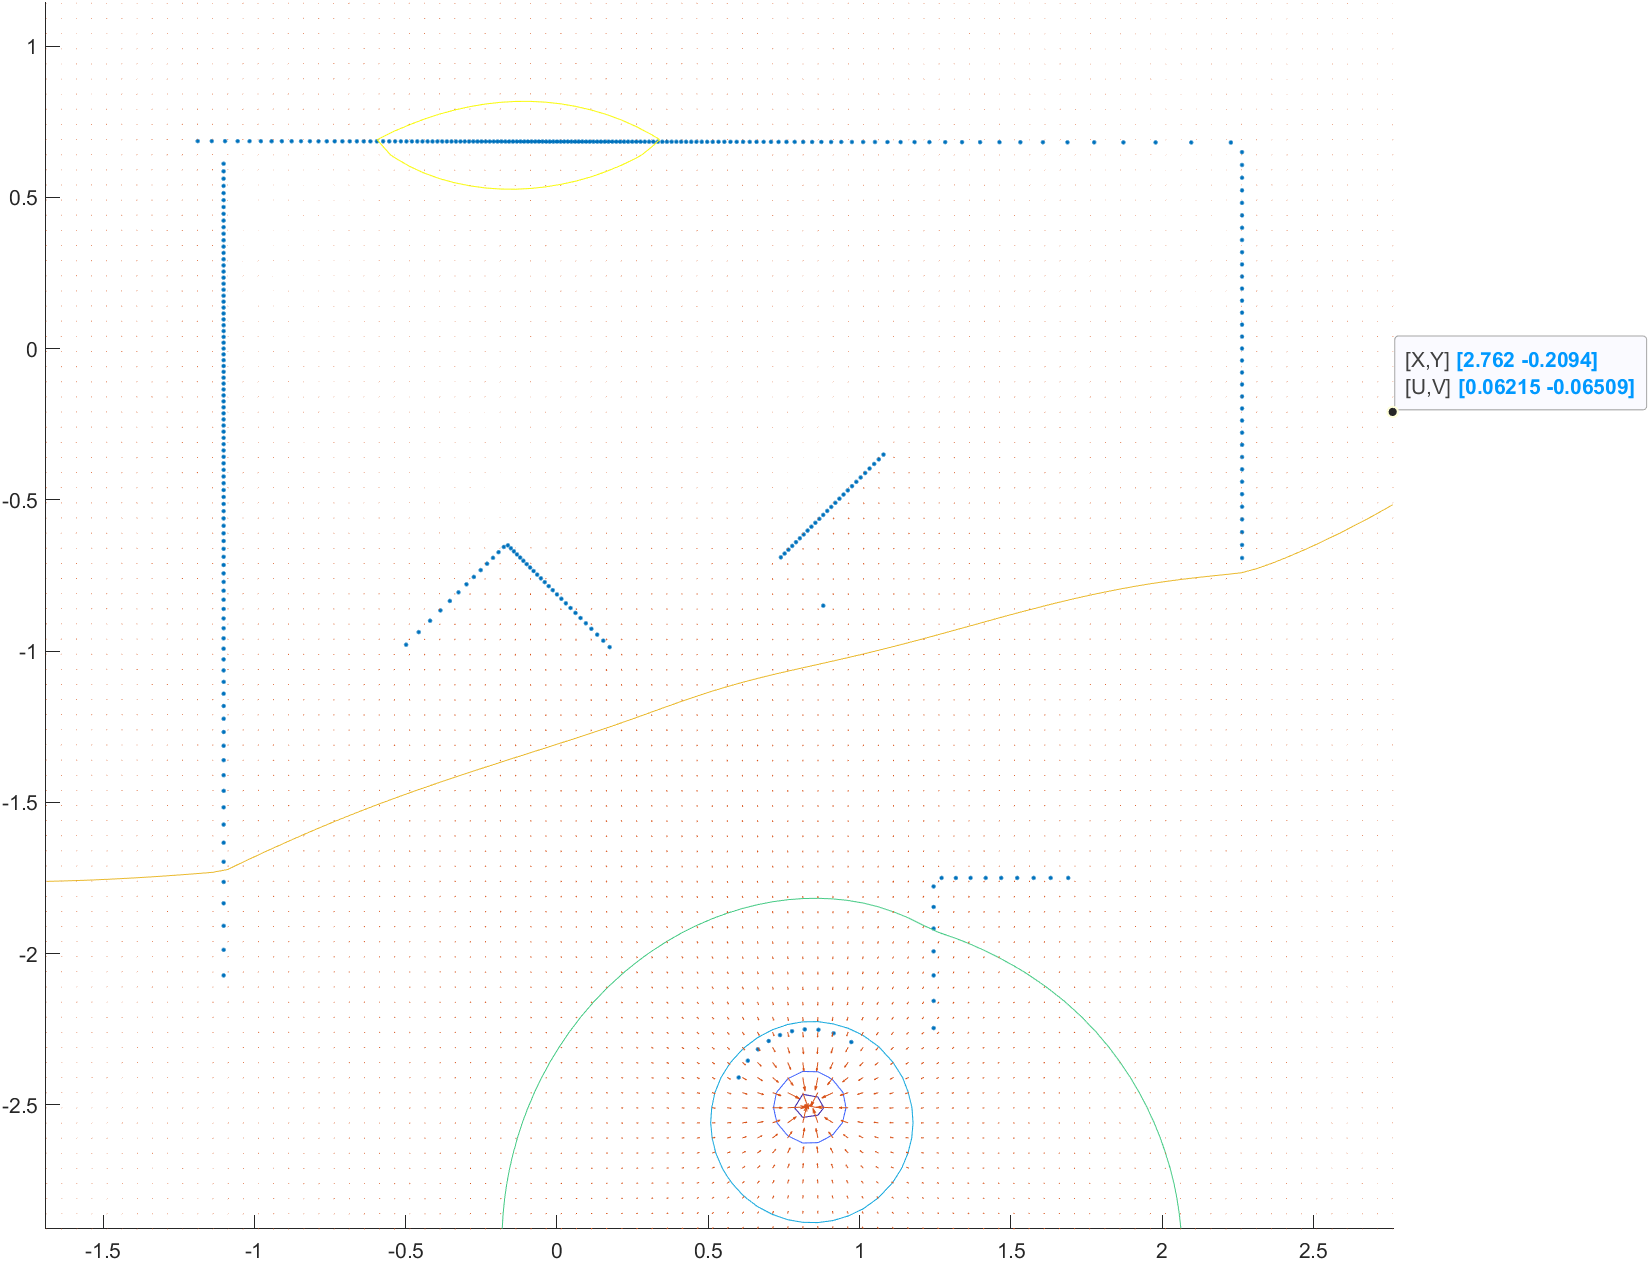
\includegraphics[width=0.65\textwidth]{img/contour_map.png}
    \caption{Contour plot of the potential field developed for the pen, based on a LIDAR scan, overlaid by the gradient of the potential field.}
    \label{fig:contourgradient}
\end{figure}

\begin{figure}[h!]
    \centering
    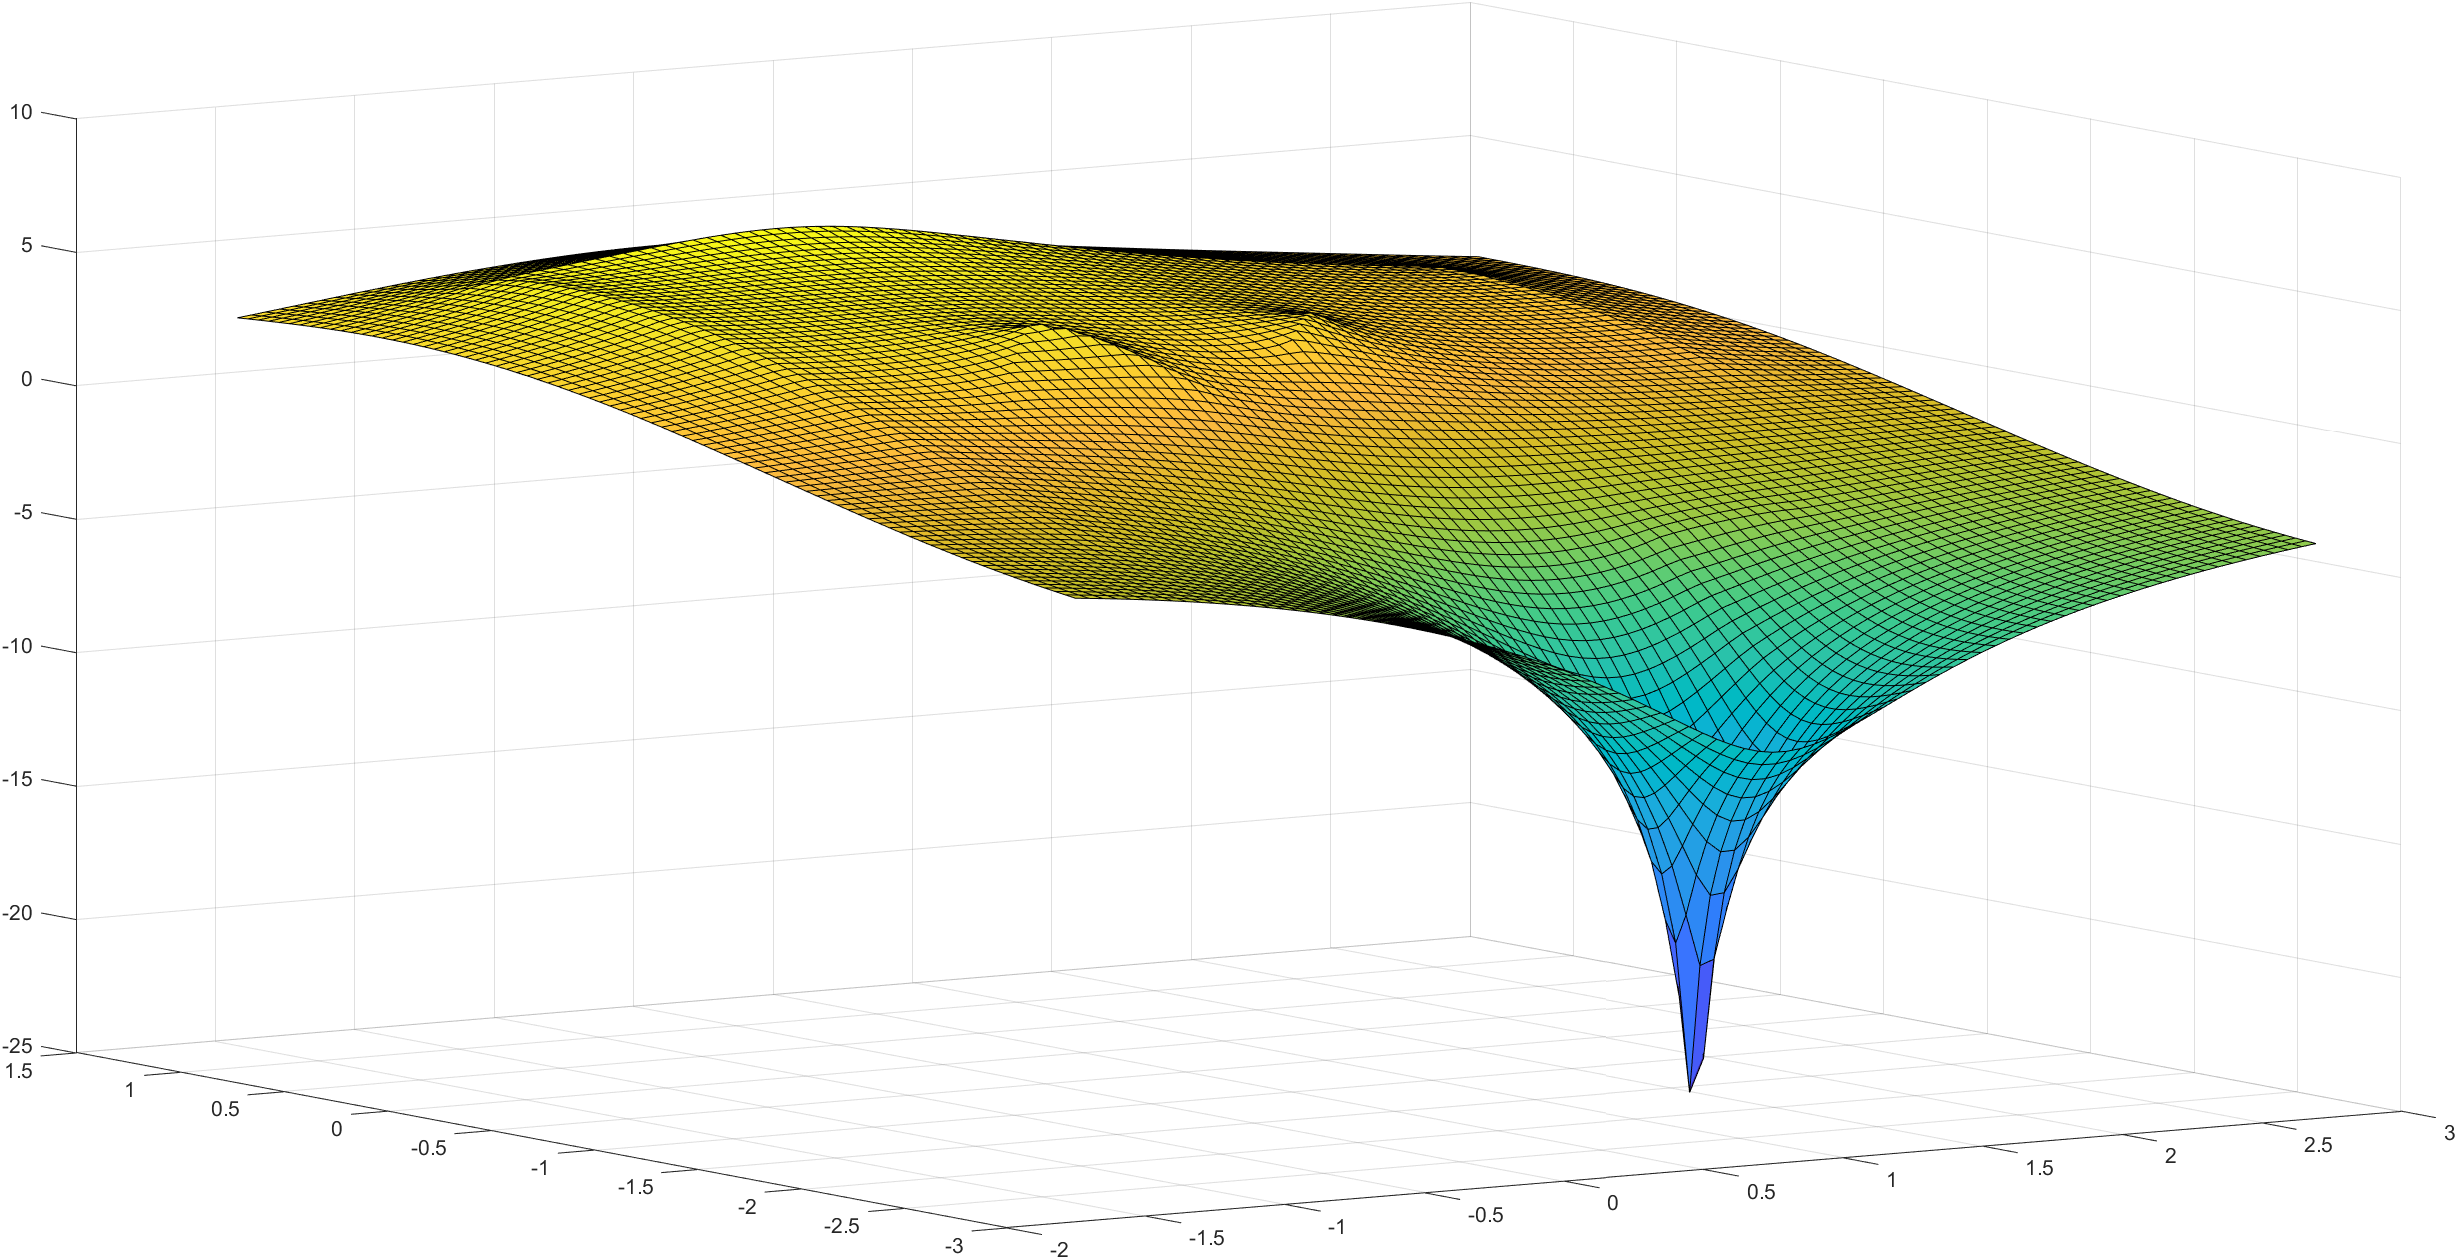
\includegraphics[width=0.65\textwidth]{img/surf.png}
    \caption{3D surface plot of the potential field developed for the pen.}
    \label{fig:surf}
\end{figure}

\pagebreak

\section{Planned Path}

\begin{figure}[htb!]
    \centering
    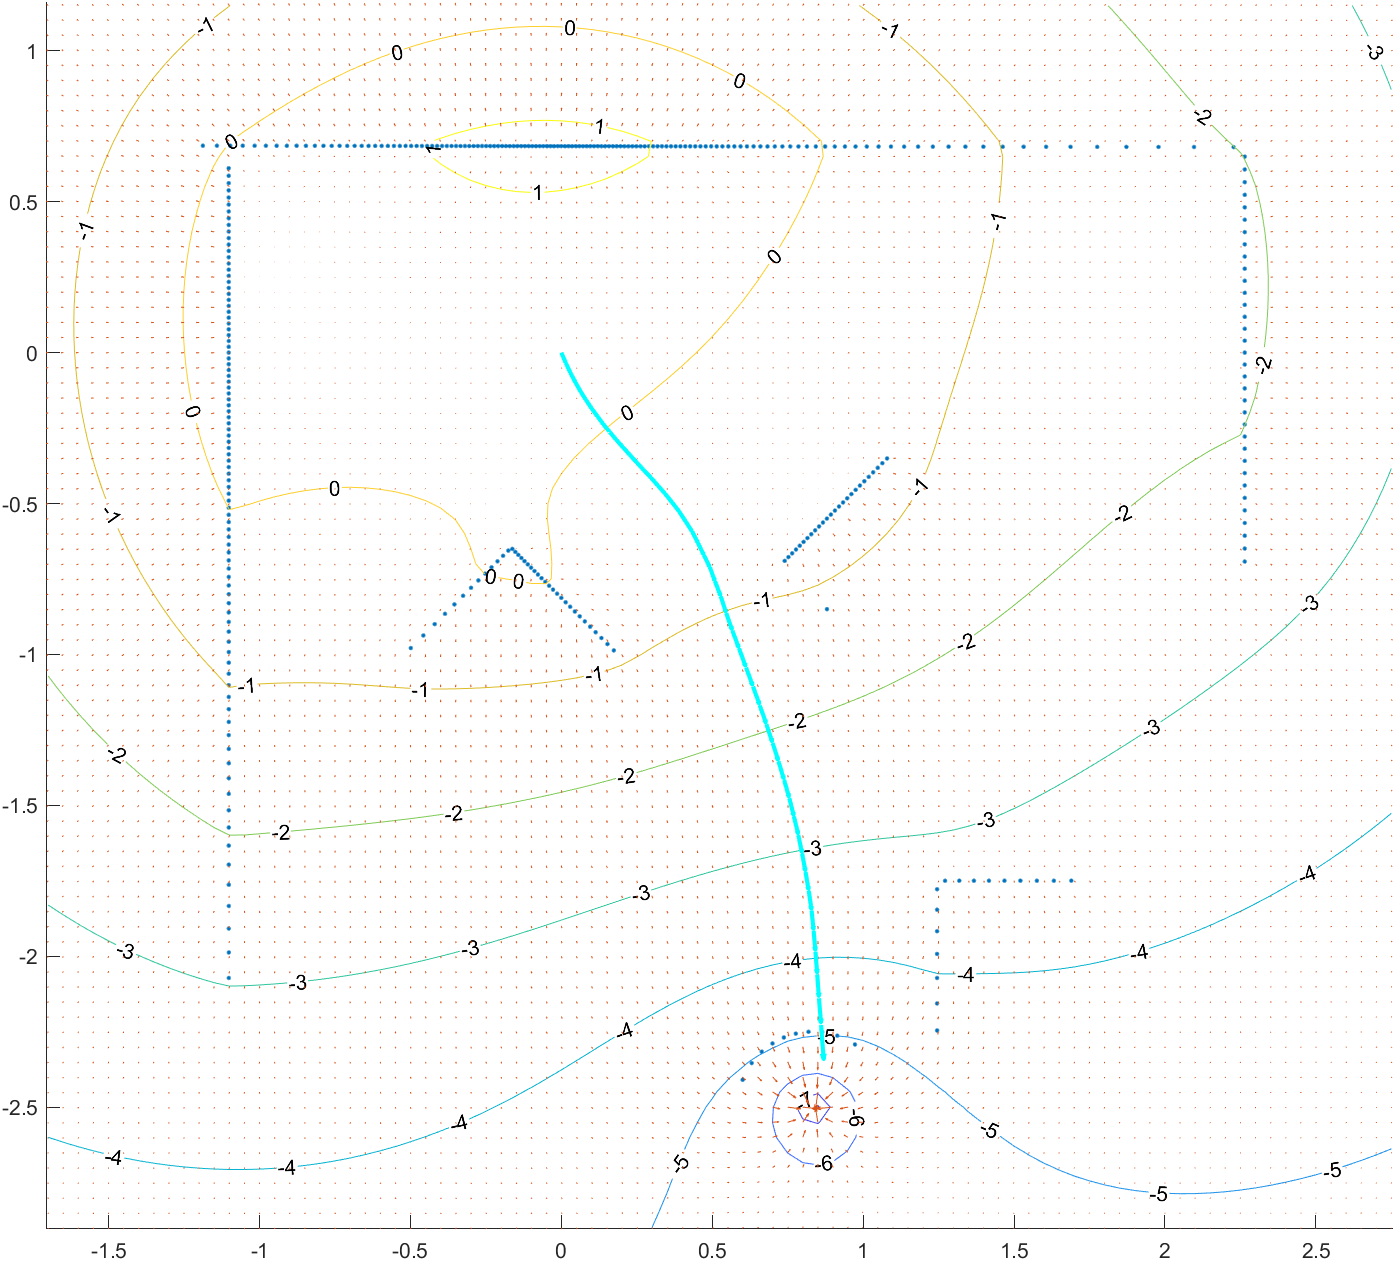
\includegraphics[width=0.5\textwidth]{img/neato_path.png}
    \caption{Planned path that the Neato will traverse through the pen.}
    \label{fig:plannedpath}
\end{figure}

\section{Code}

The code can be found here: \url{https://github.com/wsh32/qea/tree/master/pset19}


\end{document}